\section{Dynamische Systeme}

\begin{tabularx}{\columnwidth}{p{3cm}XX}
	\hline 
	\multicolumn{3}{c}{\textbf{Grundbegriffe}}\\
	\hdashline 
	
	Def. Dynamisches System & 
	\multicolumn{2}{l}{Zeitabhängiger Prozess, der durch ein mathematisches Modell beschrieben wird.}\\
	Phasenraum & \multicolumn{2}{l}{Menge aller möglichen Zustände des dynamischen Systems}\\
	Fluss & Bewegung im Phasenraum\\
	kontinuierliches System & $\bm \dot x = \bm f(\bm x), $ & $\mathbb{L}:\; t \to \bm x(t)$ (Trajektorien)\\
	diskretes System & $x_{n+1} = f(x_n)$ &  $\mathbb{L}:\; n\to x_n$\\
	\hdashline 
	\multicolumn{3}{c}{\textbf{Eindimensionale Systeme}}\\
	Lösungsmöglichkeiten & Fixpunkt, monoton steigend, monoton fallend & keine periodischen $\mathbb L$ bei autonomer DGL 1. Ordnung\\
	Fixpunkt & $f(x^*) = 0$  & $x(t) = x^*$: konstante Lösung $x^*\in \mathbb{R}$\\
	monoton steigend & $\dot x(t) > 0 \quad\forall t\in D$ & \\
	monoton fallend & $\dot x(t) < 0 \quad \forall t\in D$ & \\

	\multicolumn{3}{c}{Lineare Stabilitätsanalyse}\\
	& $\dot \eta = \eta \cdot f'(x^*) \qquad \eta(t) = \eta(0)\cdot e^{f'(x^*)\cdot t}$ & \\
	stabile Fixpunkte & nahegelegene Lösungen anziehend & $f'(x^*) < 0$\\
	instabile Fixpunkte & nahegelegene Lösungen stossen ab & $f'(x^*) > 0$\\
	unbestimmt & Stabilitätsanalyse muss von höherem Grad sein für eine Aussage& $f'(x^*) = 0$ \\

	 \hline 
	 
	 
	 \multicolumn{3}{c}{Bifurkation}\\
	 Begriffserklärung & qualitative Änderung der Dynamik eines Systems $\dot x = f(x,r)$ & $r$: freier Parameter\\
	 \hdashline 
	 Saddle-Node-Bifurkation & Fixpunkte werden durch Variation eines Systemparameters erzeugt und zerstört &  \raisebox{-\totalheight}{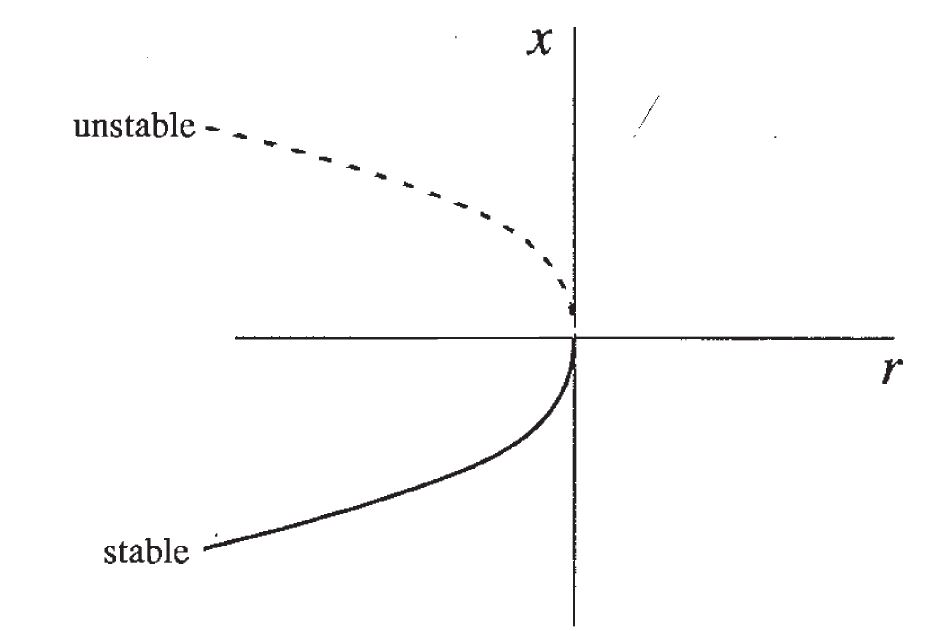
\includegraphics[scale = .15]{images/bif_saddle_node3}} \\
	 \hdashline 
	 Pitchfork-Bifurkation & \multicolumn{2}{p{14cm}}{ Bifurkation bei der ein Fixpunkt seine Stabilität ändert und zwei neue Fixpunkte entstehen.\newline Unterscheidung zwischen \textbf{Superkritisch, subkritisch}}\\
	 Superkritisch  &  
	 \begin{minipage}{6cm}
		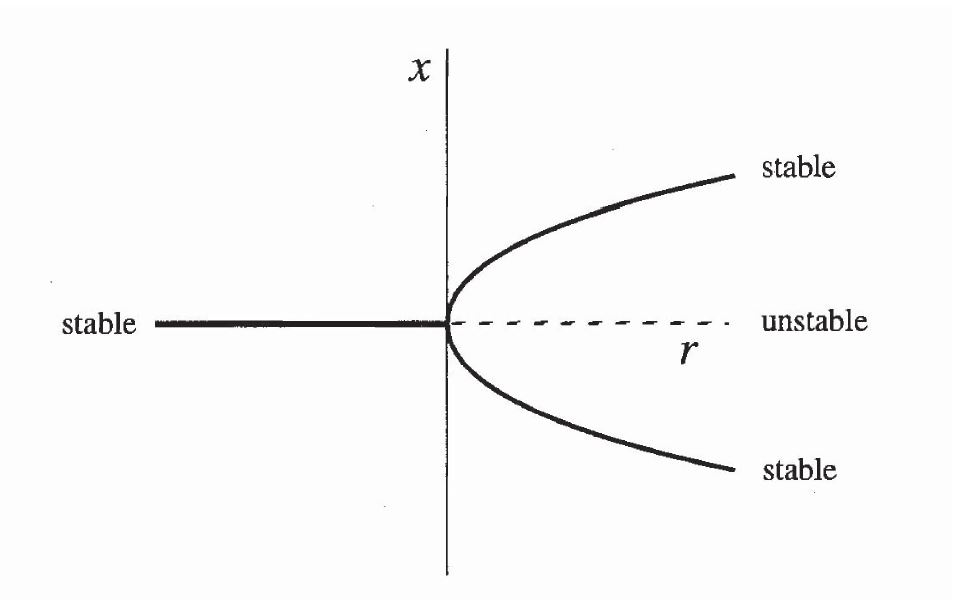
\includegraphics[scale = .15]{images/bif_superkritisch} 
	 \end{minipage}\begin{minipage}{1cm}
	  	Subkritisch
	  \end{minipage}&
		\hspace{2cm}\raisebox{-0.5\totalheight}{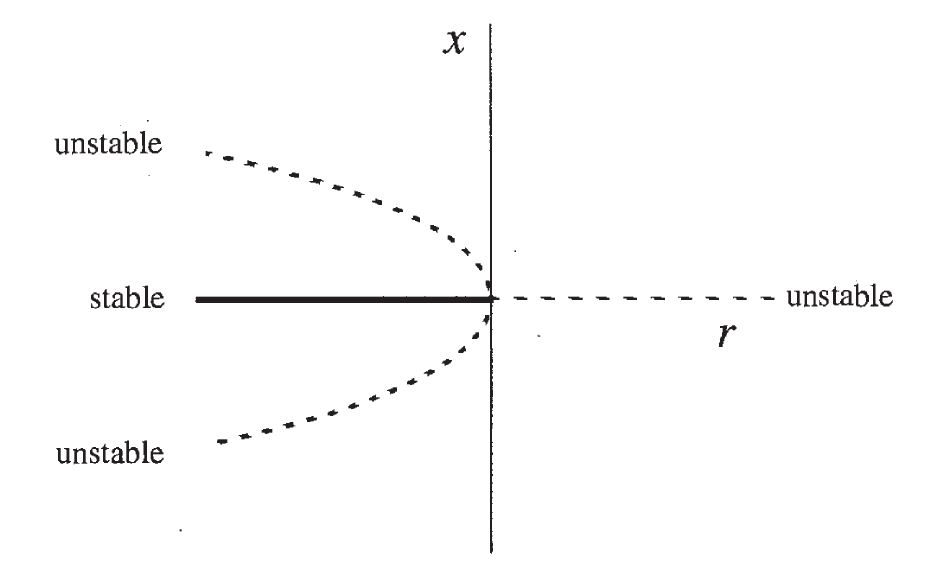
\includegraphics[scale = .15]{images/bif_subkritisch} } \\
	 \hdashline 
	 Transkritische Bifurkation & Keine Fixpunkte werden erzeugt oder vernichtet. Die Stabilität zweier Fixpunkte werden vertauscht &
	 \raisebox{-.9\totalheight}{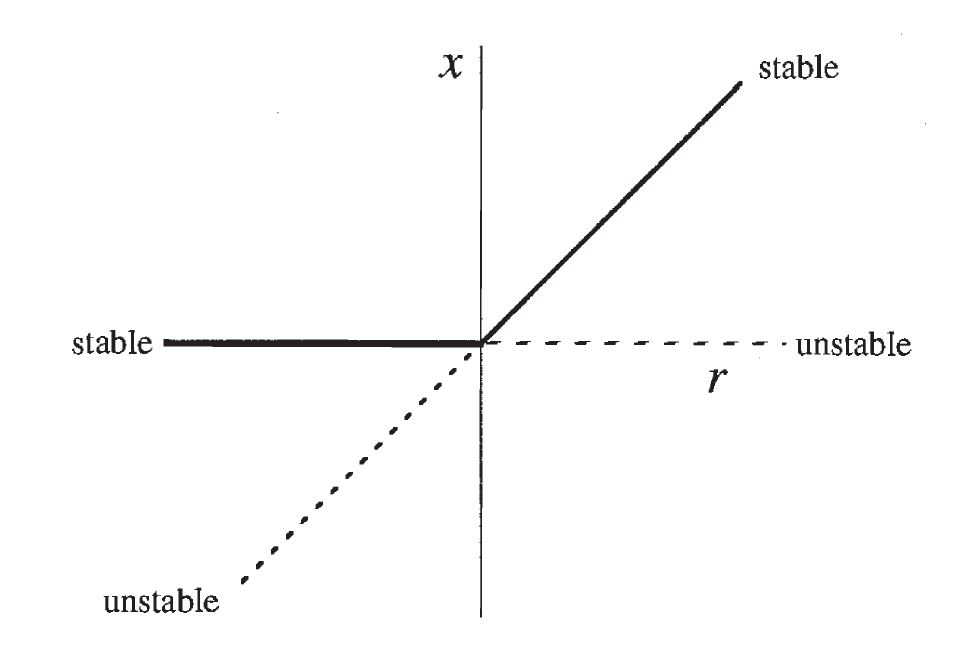
\includegraphics[scale = .15]{images/bif_transkritisch}}\\
	 \hdashline
	 Abhängigkeit mehrerer Parameter & \multicolumn{2}{l}{Es ergeben sich Kurven im Parameterraum}\\
	 \hline 
	 
 	\multicolumn{3}{c}{\textbf{Mehrdimensionale Systeme}}\\
 	\hdashline  
 	Fixpunkt & $\bm f(\bm x^*) = \bm 0$ & $\bm x^*$: Fixpunkt $\bm x^*\in \mathbb{R}^n$  \\
 	Stabilität um $\bm x^*$ &
 	konvergiert gegen $\bm x^*$ \newline entfernt sich von $\bm x^*$ & periodischer Orbit der um $\bm x^*$ kreist  \\
 	stabil & $|\bm x(t) - \bm x^*| < \epsilon_0  \qquad 0\leq t <\infty $ &alle Lösungen von $\bm x(t)$ in einer Umgebung von $\bm x^*$\\
 	asymptotisch stabil & $\lim\limits_{t\to\infty} |\bm x(t) - \bm x^*| = 0$ & asymptotisch stabil $\subseteq$ stabil \\
 	instabil & \multicolumn{2}{l}{Alle Lösungen, die die Stabilitätsbedingung nicht erfüllen} \\
 	\hdashline 
 	\multicolumn{3}{c}{Zweidimensionale Systeme}\\
 	\hdashline 
 	&$\operatorname{det}(A-\lambda I) = 0 \; \implies \boxed{\lambda^2-\tau\lambda + \Delta = 0}$&
 	$\tau = \operatorname{tr}(a) = a_{11} + a_{22}$\newline 
 	$\Delta = \operatorname{det}(A) = a_{11}a_{22} - a_{12}a_{21}$\\
 	
 	&
 	$\lambda_{1,2} = \dfrac{1}{2}\left(\tau \pm \sqrt{\tau^2 - 4\Delta}\right)$ & 
 	  $\tau = \lambda_1 + \lambda_2$ \newline $\Delta = \lambda_1\lambda_2$ \\
 	  Sattelpunkt & $\Delta < 0,\quad \lambda_1 < 0 < \lambda_2$ oder $\lambda_2 < 0 < \lambda_1$&\\
 	  \hdashline 
 	   \multicolumn{3}{l}{$\Delta > 0, \quad \tau < 0\implies \quad \operatorname{Re}(\lambda_1) > 0, \quad \operatorname{Re}(\lambda_2) < 0$} \\
 	  \multicolumn{3}{p{\columnwidth}}{stabiler Knotenpunkt:  $\tau^2 - 4\Delta \geq 0, \quad \lambda_{1,2} \in \mathbb{R}$  \newline 
 	  stabiler Strudelpunkt:   $\tau^2 - 4\Delta < 0, \quad\lambda_{1,2} \not\in \mathbb{R}$ } \\
 	\hdashline 
	   \multicolumn{3}{l}{$\Delta > 0, \quad \tau > 0\implies\quad \operatorname{Re}(\lambda_1) > 0, \quad \operatorname{Re}(\lambda_2) > 0$}\\
	   \multicolumn{3}{p{\columnwidth}}{instabiler Knotenpunkt:  $\tau^2 - 4\Delta \geq 0, \quad \lambda_{1,2} \in \mathbb{R}$  \newline 
	   instabiler Strudelpunkt:   $\tau^2 - 4\Delta < 0, \quad\lambda_{1,2} \not\in \mathbb{R}$ } \\
	  \hdashline 
 	 Zentrum, elliptischer Fixpunkt & \multicolumn{2}{p{14cm}}{ad $\Delta > 0, \quad \tau = 0\implies\quad \operatorname{Re}(\lambda_1)= \operatorname{Re}(\lambda_2)  = 0$}\\
 	 \hdashline 
 	  degenerierten System & $\Delta = 0 \implies \quad \lambda_1 = \lambda_2 = 0$ & \\
 	  \hdashline 
	 \multicolumn{2}{l}{asymptotisch stabil: $\operatorname{Re}(\lambda_i) < 0\qquad $  stabil: $\operatorname{Re}(\lambda_i) \leq 0 \qquad $ instabil: $\operatorname{Re}(\lambda_i) > 0$}\\
	 \hdashline 
\end{tabularx}